\section{Introduction}
\label{sec:intro}

\begin{comment}
Motivation:
- Counterfactual is important. Used in many evaluation and model improvement approaches. Like mentioned in other papers, perturbations of inputs would allow us to highlight what really matters more efficiently than getting different examples
- Existing methods have limitations:
	○ Auto-method seems to focus on word substitution, or paraphrasing. More scalable, but usually too simplistic.
	○ More diverse counterfactuals rely on human effort. More diverse and natural, but hard to scale:
		§ Cannot create this for all instances
		§ For just one instance, just getting one perturbation (good -> bad) still ignores many other decision boundary dimensions (good -> not good)
	- Goal: To create a counterfactual generator that
		○ can automatically cover more patterns
		○ But still systematic enough for scaled analysis

Contribution bullets:
	- Survey on prior work, summarize applications + desired properties
	- Perturbation as a generation model, the design of perturbation type control and the importance of [BLANK]
	- Application - counterfactual explanation
		○ Design - categorize patterns to search for, grouping/ranking/summarization, interactive mode
		○ Validly - User study
		○ Finding - case study on some model
	- Application - labeling
		○ Ranking, grouped labeling
		○ Training data: get better results compared to
			§ Adding the same amount of training data
			§ asking people to generate counterfactuals using the same budget
		○ Evaluation data: further decrease the SOTA model performance
		○ Vision - not tested, but we think presenting some existing perturbations first should help people get more creative when they come up with their owns [future work…]

\end{comment}



Researchers and practitioners expect NLP models to learn linguistic patterns, yet language is too high dimensional for any datasets to exhaust.
Due to annotation artifacts~\cite{}, models usually learn spurious correlations that are hard to detect with test datasets, who have similar biases as the training set~\cite{rajpurkar-etal-2018-know}.
%Compared to random data, various work has found that 
To inspect and improve models' decision boundaries, various work has explored perturbing existing datasets, rather than adding new random data.
The intuition is, paired data points can more effectively reveal unlearned phenomena. 


However, these approaches have their limitations. 
Auto-method focus on word substitution, or paraphrasing. While they are more scalable, they usually cover simplistic or limited number of perturbations.
More diverse perturbations rely on human effort, but becomes hard to scale to more instances.
Prior work usually cover For just one instance, just getting one perturbation (good -> bad) still ignores many other decision boundary dimensions (good -> not good). \wts{Add a figure.}

In this work, we explore the automated perturbation generation.
We survey existing papers on applications of perturbations, and summarize that a perturbation generator should automatically cover various patterns, but are still controlled enough to allow targeted changes (for pattern-specific data augmentation or model analysis.)
We formalize the perturbation as a generative task, and instantiate the generator by finetuning language models.
Rather than using it for completing XXXX, we design the training prompts such that models like GPT-2 learn to generate the perturbation after seeing the original sentence.


For each pair, we generate the training prompt such that:
(1) The prompt concatenates the original sentence and the new one;  
(2) The prompt uses a fill-in-the-blank structure~\cite{}, that determines \emph{where} to change (based on linguistic features like part-of-speech tagging or dependency trees);
(3) The prompt contains \tagstrs that directs \emph{how} to change a sentence, which we summarize based on existing papers on perturbations.
To help the model learn different \tagstrs, we combine six existing datasets for the finetuning.
All datasets contain paired sentences that can be viewed as minimal perturbations of each other, but cover different \tagstrs.
As a result, in Figure~\ref{} to test the impact of negation, one can say \emph{``add negation modifiers to aux.''}\wts{Add figure.}
%, instead of enumerating rules like \swap{did}{didn't}, \swap{\texttt{VERB}}{would never \texttt{VERB}}

\begin{figure}[t]
\centering
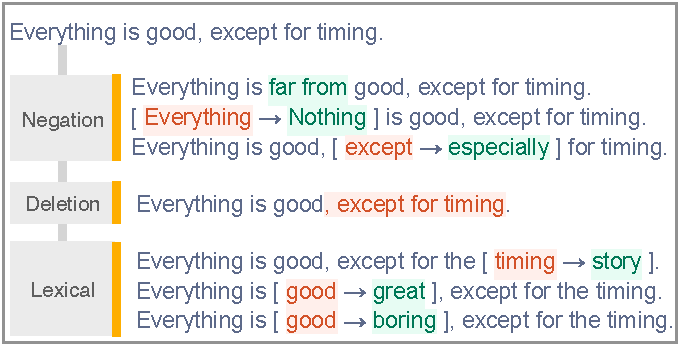
\includegraphics[width=1\columnwidth]{figures/teaser}
\vspace{-15pt}
\caption{Teaser of the idea. \wts{Placeholder; Probably shouldn't be just examples, given we already have a big table. Re-do to include the applications.}}
\vspace{-10pt}
\label{fig:mturk_instruction}
\end{figure}


We demonstrate the usefulness of \sysname in three applications. 
First, we verify that the perturbations is beneficial for training and evaluation data collection. 
In three NLP tasks --- sentiment analysis (\sst), duplicate question detection (\qqp), and natural language inference (\nli) --- we ask crowdworkers to label the generated multiple perturbations of the same original instance.
We observed that the labeling was more efficient than not only creating new perturbation examples, but also labeling new instances, as workers only need to parse the entire example once, and then process the labeling based on the changes.
\wts{Do we need to claim this, and do we need to verify this? Or maybe we can just say this is true in the labeling part, and do not claim *observing* it?}
Using the collected data as contrast sets~\cite{}, \ie evaluation dataset with minimal perturbations across the decision boundary, we observed that the performances of state-of-the-art models decrease significantly. 
Using the data for augmentation, we observed that the perturbation helps improve models' generalization accuracies on out-of-domain datasets, challenge sets and contrast sets, as well as CheckList testing results~\cite{checklist:acl20}, while maintaining the in-domain accuracy.

Second, we also use the perturbations to supply existing explanations methods.
We ``critisize'' existing feature attribution methods like SHAP~\cite{} or LIME~\cite{} by selecting perturbations whose model prediction conflict with the corresponding token importance (\eg the model prediction changes when a supposedly insignificant feature is replaced.)
In a user study, we verify the surprise...

In summary, we contribute: 
\begin{compactenum}
\item A formalization of the perturbation task, with applications and desire properties extracted from existing literature.
\item A finetuned language model as perturbation generator, with 
\item demonstrations of perturbation usefulness on data augmentation, contrast set collection, and model explanation. 
\end{compactenum}


   


%Automated approahces using templates or word substitutions usually cover limited capabilities, whereas manual perturbations are usually expensive and hard to scale. 


%Another approach is to employ counterfactual reasoning: what would have happened if X was different? Many analysis and evaluation approaches rely on counterfactual reasoning, e.g. anchors, Errudite, SEARs, contrast sets, 'learning the difference that makes a difference', and counterfactual explanations in general. Some data augmentation approaches also rely on counterfactual reasoning, and focus on perturbing existing inputs rather than on getting new data. Intuitively, perturbations of inputs would allow us to highlight what really matters more efficiently than getting different examples (again, language is high dimensional).


\begin{comment}

prior work on counterfactual generation typically follows one of two extremes.
On the one hand, templates or perturbation rules (used by Errudite and Checklist) allow targeted inspections, but can only cover limited linguistic patterns.
On the other hand, those that thrive in diversity are either too uncontrolled (e.g., text generation~\cite{iyyer2018adversarial}) or hard to scale (e.g., manual rewrites~\cite{kaushik2019learning, gardner2020contrast}).



I seek to achieve a balance between control and generation diversity. 
To this end, I have fine-tuned language models for perturbation generation.

%Through intrinsic evaluation, we have found that our method works as we expect.
Moving forward, I plan to explore whether our method is helpful in various downstream tasks. 
First, the perturbations can potentially serve as extensive counterfactual explanations, i.e., explaining models' reaction to \emph{a set of changes}, rather than \emph{one change}~\cite{ribeiro2018semantically, ribeiro2018anchors, feder2020causalm}.
%We plan to use groups of perturbations as explanations, and suggests insightful groups to the practitioner based on certain predefined criteria.
A group of highly related changes may reveal model insufficiencies that are hard to spot otherwise (e.g., sentiment analysis model only recognizing certain kinds of negations like ``did not'', but misclassifying others like ``I would never.'')
%We plan to design a mixed-initiative method, where a system ranks groups of perturbations based on certain predefined criteria, and suggests the most insightful ones to the practitioner. 
%For example, minimal changes that affected the models' prediction possibly indicate the model is unstable.
%In turn, the practitioner can customize the exploration based on where or how s/he would like to inspect the model, and decide when to move to a different angle, or further drill down.
We plan to verify the insightfulness of these explanations through typical evaluation methods, e.g., surprise, simulatability~\cite{hase2020evaluating}.
Second, I hope to collect more effective contrast sets~\cite{gardner2020evaluating} that can reveal the vulnerability of the model.
I plan to annotate the generated perturbations with class labels in crowdsourcing tasks (e.g., positive or negative in sentiment analysis). 
%where a crowdworker label each sentence with a .%, or invalid (the sentence does not make sense, etc.). 
Then, to evaluate, I plan to verify whether we can find more bugs in the state-of-the-art models (i.e., if the accuracy further drops on these datasets).
Further, the data collected can be used for data augmentation~\cite{kaushik2019learning}. 
I plan to explore whether models trained with such perturbations can become more capable of handling certain capabilities (e.g., pass more tests in CheckList related to negation).
\end{comment}

